\documentclass[12pt]{article}

\usepackage{amsfonts}
\usepackage{amsmath}
\usepackage{amssymb}
\usepackage{cite}
\usepackage{enumerate}
\usepackage{fancyhdr}
\usepackage[headheight=1in,margin=1.25in]{geometry}
\usepackage[colorlinks=true,linkcolor=blue]{hyperref}
\usepackage{mathtools}
\usepackage{scalerel}
\usepackage{setspace}

\usepackage{tikz}

\newcommand{\N}{\ensuremath{\mathbb{N}}}
\newcommand{\Z}{\ensuremath{\mathbb{Z}}}
\newcommand{\Q}{\ensuremath{\mathbb{Q}}}
\newcommand{\R}{\ensuremath{\mathbb{R}}}
\newcommand{\C}{\ensuremath{\mathbb{C}}}

\newcommand{\e}{\ensuremath{\varepsilon}}
\renewcommand{\d}{\ensuremath{\delta}}

\newcommand{\angleb}[1]{\left\langle#1\right\rangle}
\newcommand{\braceb}[1]{\left\{#1\right\}}
\newcommand{\bracketb}[1]{\left[#1\right]}
\newcommand{\parenb}[1]{\left(#1\right)}
\newcommand{\vertb}[1]{\left\vert#1\right\vert}
\newcommand{\dvertb}[1]{\left\Vert#1\right\Vert}

\DeclarePairedDelimiter\floor{\lfloor}{\rfloor}
\DeclarePairedDelimiter\ceil{\lceil}{\rceil}

\renewcommand{\Re}{\text{Re}}
\renewcommand{\Im}{\text{Im}}

\newcommand{\comp}{\complement}
\newcommand{\sdiff}{\setminus}

\newcommand{\solution}{\textit{Solution: }}
\newcommand{\proof}{\textit{Proof: }}
\newcommand{\partialdone}{\ensuremath{\strut\hfill\blacktriangle}}
\newcommand{\done}{\ensuremath{\strut\hfill\blacksquare}}

\newcommand{\mc}[1]{\ensuremath{\mathcal{#1}}}

\renewcommand{\t}[1]{\text{ #1 }}
\newcommand{\impl}{\ensuremath{\implies}}
\newcommand{\sectionskip}{\vspace{0.15in}}
\newcommand{\tri}{\triangle}
\newcommand{\ovl}[1]{\ensuremath{\overline{#1}}}

\newcommand{\longdiv}{
	\smash{
		\mkern-0.43mu\vstretch{1.31}{\hstretch{.7}{)}}
		\mkern-5.2mu\vstretch{1.31}{\hstretch{.7}{)}}
	}
}

\begin{document}

\pagestyle{fancy}
\fancyhead[L]{Ahlfors}
\fancyhead[C]{Complex Analysis}
\fancyhead[R]{Chapter 1}

\setlength{\parindent}{0in}
\setlength{\parskip}{0.1in}
\setstretch{1}

\section*{Section 1.1}

\textbf{1)} Represent the following values in the form \( a + bi \), where
\( a, b \in \R\).
\[
	(1 + 2i)^3, \quad
	\frac{5}{-3 + 4i}, \quad
	\parenb{ \frac{2 + i}{3 - 2i} }^2, \quad
	(1 + i)^n + (1 - i)^n
\]
In this case, we assume \( n \in \N_0 \).

\solution
\[ (1 + 2i)^3 = (-3 + 4i)(1 + 2i) = \boxed{-11 - 2i} \]
\[
	\frac{5}{-3 + 4i} =
	\frac{5}{-3 + 4i} \cdot \frac{-3 - 4i}{-3 - 4i} =
	\frac{-15 - 20i}{25} =
	\boxed{-\frac{3}{5} - \frac{4}{5}i}
\]
\[
	\parenb{\frac{2 + i}{3 - 2i}}^2 =
	\frac{2 + i}{3 - 2i} \cdot \frac{2 + i}{3 - 2i} =
	\frac{3 + 4i}{5 - 12i} =
	\frac{3 + 4i}{5 - 12i} \cdot \frac{5 + 12i}{5 + 12i} =
	\frac{-33 + 56i}{169}
\]
\[ = \boxed{-\frac{33}{169} + \frac{56}{169}i} \]

Using the binomial theorem, we see that
\[
	(1 + i)^n + (1 - i)^n
	= \sum_{k = 0}^n \binom{n}{k}i^k + \sum_{k = 0}^n \binom{n}{k}(-i)^k
	= \sum_{k = 0}^n \binom{n}{k} \bracketb{i^k + (-i)^k}.
\]
Since \( i = (-i)^3 \) and \( -i = i^3 \), we have that
\( i^k + (-i)^k = 0 \) for odd \( k \), thus it suffices to consider the even
terms of the sum.
Additionally, since \( i^2 = (-i)^2 = -1 \) and \( i^4 = (-i)^4 = 1 \), we have
\( i^k + (-i)^k = 2(-1)^k \) for even \( k \).
This gives us
\[
	(1 + i)^n + (1 - i)^n
	= \boxed{\sum_{k = 0}^{\floor{n/2}} \binom{n}{2k} 2(-1)^{2k}}
\]
and thus we obtain a real number for all values of \( n \).

\textbf{2)} Letting \( z = a + bi \) for \( a,b \in \R \), find the real and
imaginary parts for the following complex numbers:
\[
	z^4, \quad
	\frac{1}{z}, \quad
	\frac{z - 1}{z + 1}, \quad
	\frac{1}{z^2}
\]

\solution
\[
	z^4 = (a + bi)^4 = (a + bi)^2 (a + bi)^2 = (a^2 + 2abi - b^2)^2
\]
\[
	= \boxed{a^4 - 6a^2b^2 + b^4 + (4a^3b  - 4ab^3)i}
\]
\[
	\frac{1}{z} = \frac{1}{a + bi} \cdot \frac{a - bi}{a - bi}
	= \frac{a - bi}{a^2 + b^2}
	= \boxed{\frac{a}{a^2 + b^2} - \frac{b}{a^2 + b^2}i}
\]
\[
	\frac{z - 1}{z + 1} = \frac{a - 1 + bi}{a + 1 + bi}
	\cdot \frac{a + 1 - bi}{a + 1 - bi}
	= \frac{(a - 1 + bi)(a + 1 - bi)}{(a + 1)^2 + b^2}
	= \frac{a^2 + b^2 - 1 + 2bi}{(a + 1)^2 + b^2}
\]
\[
	= \boxed{
		\frac{a^2 + b^2 - 1}{(a + 1)^2 + b^2}
		+ \frac{2b}{(a + 1)^2 + b^2}i
	}
\]
\[
	\frac{1}{z^2} = \frac{1}{(a + bi)^2} = \frac{1}{a^2 - b^2 + 2abi}
	= \frac{1}{a^2 - b^2 + 2abi}
	\cdot \frac{a^2 - b^2 - 2abi}{a^2 - b^2 - 2abi}
\]
\[
	= \frac{a^2 - b^2 - 2abi}{a^4 + 2a^2b^2 + b^4}
	= \boxed{
		\frac{a^2 - b^2}{(a^2 + b^2)^2} - \frac{2ab}{(a^2 + b^2)^2}i
	}
\]

\textbf{3)} We have that
\[
	\parenb{\frac{-1 \pm i\sqrt{3}}{2}}^3
	= \parenb{\frac{\pm 1 \pm i\sqrt{3}}{2}}^6
	= 1
\]
for all combinations of \( + \) and \( - \) with the \( \pm \) signs.

\textit{Proof:}
Interpreting the complex numbers inside the parentheses as points in
\( \R^2 \), we see that they lie on the unit circle for all possible
combinations of \( + \) and \( - \).
The following picture demonstrates this:

\begin{center}
	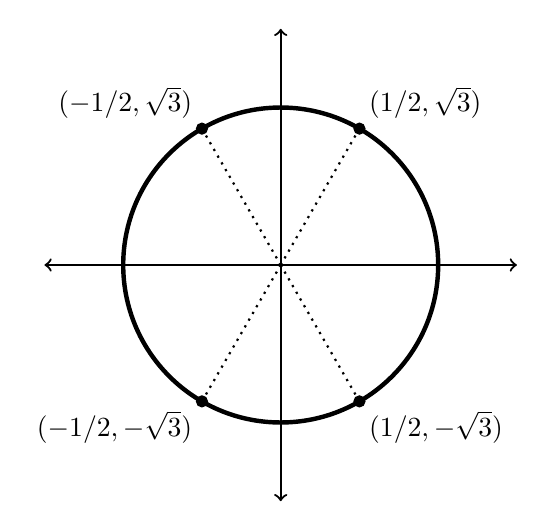
\begin{tikzpicture}[scale=2]
		% axes
		\draw [<->,thick] (0,1.5) -- (0,0) -- (1.5,0);
		\draw [<->,thick] (0,-1.5) -- (0,0) -- (-1.5,0);

		% unit circle
		\draw [ultra thick] (0,0) circle [radius=1];

		% points
		\draw [fill] (0.5,0.866) circle [radius=1pt];
		\draw [dotted,thick] (0,0) -- (0.5,0.866);
		\node [above right] at (0.5,0.866) {\( (1/2, \sqrt{3}) \)};

		\draw [fill] (-0.5,0.866) circle [radius=1pt];
		\draw [dotted,thick] (0,0) -- (-0.5,0.866);
		\node [above left] at (-0.5,0.866) {\( (-1/2, \sqrt{3}) \)};

		\draw [fill] (0.5,-0.866) circle [radius=1pt];
		\draw [dotted,thick] (0,0) -- (0.5,-0.866);
		\node [below right] at (0.5,-0.866) {\( (1/2, -\sqrt{3}) \)};

		\draw [fill] (-0.5,-0.866) circle [radius=1pt];
		\draw [dotted,thick] (0,0) -- (-0.5,-0.866);
		\node [below left] at (-0.5,-0.866) {\( (-1/2, -\sqrt{3}) \)};
	\end{tikzpicture}
\end{center}
Since multiplication of two complex numbers adds their angles and multiplies
their magnitudes, it is easy to see that the equation holds.
\done

\section*{Section 1.2}

\textbf{1)}
Compute the values of the following complex square roots:
\[
	\sqrt{i}, \quad
	\sqrt{-i}, \quad
	\sqrt{1 + i}, \quad
	\sqrt{\frac{1 - i\sqrt{3}}{2}}
\]

\solution
We use the following formula to compute \( \sqrt{a + bi} \):
\[
	\sqrt{a + bi}
	= \pm\parenb{
		\sqrt{\frac{a + \sqrt{a^2 + b^2}}{2}}
		+ i \frac{b}{\vertb{b}} \sqrt{\frac{-a + \sqrt{a^2 + b^2}}{2}}
	}
\]
This results in the following values:
\[
	\sqrt{i} = \boxed{\pm\parenb{\frac{1}{\sqrt{2}} + \frac{1}{\sqrt{2}}i}}
	\kern0.025in,\kern0.15in
	\sqrt{-i} = \boxed{\pm\parenb{\frac{1}{\sqrt{2}} - \frac{1}{\sqrt{2}}i}}
	\kern0.025in,
\]
\[
	\sqrt{1 + i} = \boxed{
		\pm\parenb{
			\sqrt{\frac{1 + \sqrt{2}}{2}}
			+ i \sqrt{\frac{-1 + \sqrt{2}}{2}}
		}
	}\kern0.025in,
\]
\[
	\sqrt{\frac{1 - i\sqrt{3}}{2}}
	= \sqrt{\frac{1/2 + \sqrt{1/4 + 3/4}}{2}}
	- i\sqrt{\frac{-1/2 + \sqrt{1/4 + 3/4}}{2}}
	= \boxed{\pm\parenb{\frac{\sqrt{3}}{2} - \frac{1}{2}i}}
\]

\textbf{2)}
Find all four values of \( \sqrt[4]{-1} \).

\solution
We first consider the values of \( \sqrt{-1} \), which happen to be
\( \pm i \).
Since \( \sqrt[4]{-1} = \sqrt{\sqrt{-1}} = \sqrt{\pm i} \), we have that the
four values of \( \sqrt[4]{-1} \) are given as follows:
\[
	\boxed{
		\pm\parenb{\frac{1}{\sqrt{2}} + i\frac{1}{\sqrt{2}}}
		\kern-0.05in,\kern0.075in
		\pm\parenb{\frac{1}{\sqrt{2}} - i\frac{1}{\sqrt{2}}}
	}
\]

\textbf{3)}
Find all four values of \( \sqrt[4]{i} \) and \( \sqrt[4]{-i} \).

\solution
Recalling the previously determined values for \( \sqrt{i} \) and
\( \sqrt{-i} \), we find \( \sqrt[4]{i} \) and \( \sqrt[4]{-i} \) as
follows:
\[
	\sqrt[4]{i}
	= \sqrt{\sqrt{i}}
	= \sqrt{\pm\parenb{\frac{1}{\sqrt{2}} + i\frac{1}{\sqrt{2}}}}
\]
\[
	= \boxed{
		\pm\parenb{
			\sqrt{\frac{2 + \sqrt{2}}{4}} + i\sqrt{\frac{2 - \sqrt{2}}{4}}
		}
		\kern-0.05in,\kern0.075in
		\pm\parenb{
			\sqrt{\frac{2 - \sqrt{2}}{4}} + i\sqrt{\frac{2 + \sqrt{2}}{4}}
		}
	}\kern0.025in,
\]
\[
	\sqrt[4]{-i}
	= \sqrt{\sqrt{-i}}
	= \sqrt{\pm\parenb{\frac{1}{\sqrt{2}} - i\frac{1}{\sqrt{2}}}}
\]
\[
	= \boxed{
		\pm\parenb{
			\sqrt{\frac{2 + \sqrt{2}}{4}} + i\sqrt{\frac{2 - \sqrt{2}}{4}}
		}
		\kern-0.05in,\kern0.075in
		\pm\parenb{
			\sqrt{\frac{2 - \sqrt{2}}{4}} + i\sqrt{\frac{2 + \sqrt{2}}{4}}
		}
	}
\]

\textbf{4)}
Given \( a, b \in \C \), solve the following quadratic equation for \( z \):
\[
	z^2 + az + b = 0
\]

\solution
We can complete the square as follows:
\[
	z^2 + az = (z + a/2)^2 - a^2/4 = -b,
\]
and since square roots of complex numbers are defined, we can solve for
\( z \) as follows:
\[
	z = \pm\sqrt{\frac{a^2}{4} - b} - \frac{a}{2}
	= \frac{-a \pm 2\sqrt{a^2/4 - b}}{2}
	= \frac{-a \pm \sqrt{a^2 - 4b}}{2},
\]
which is equivalent to the standard real valued quadratic equation for monic
quadratic polynomials.

\section*{Section 1.3}

\textbf{1)}
Let \( F \) be set of all matrices in \( \R^{2 \times 2} \) that take the form
\[
	\begin{bmatrix*}[r]
		a & b \\ -b & a
	\end{bmatrix*}
	\kern-0.025in,
\]
then \( F \) is a field under the operations of matrix addition and
multiplication, and furthermore is isomorphic to \C.

\proof
The zero matrix and the identity matrix act as the 0 and 1 of \( F \),
respectively.
It is also easy to verify that \( F \) is closed under addition and
multiplication.
We additionally have that
\[
	\begin{bmatrix*}[r]
		-a & -b \\ b & -a
	\end{bmatrix*}
	\hspace{0.1in}\text{and}\hspace{0.1in}
	\begin{bmatrix*}[r]
		a/(a^2 - b^2) & b/(a^2 - b^2) \\
		-b/(a^2 - b^2) & a/(a^2 - b^2)
	\end{bmatrix*}
\]
serve as the additive and multiplicative inverses respectively.
Finally,
\[
	\begin{bmatrix*}[r]
		a & b \\ -b & a
	\end{bmatrix*}
	\begin{bmatrix*}[r]
		c & d \\ -d & c
	\end{bmatrix*}
	= \begin{bmatrix*}[r]
		ac - bd & ad + bc \\ -ad - bc & ac - bd
	\end{bmatrix*}
	= \begin{bmatrix*}[r]
		c & d \\ -d & c
	\end{bmatrix*}
	\begin{bmatrix*}[r]
		a & b \\ -b & a
	\end{bmatrix*}
	\kern-0.025in,
\]
which verifies the commutativity of \( F \).

Having shown that \( F \) is a field, we turn our attention to the function
\( \phi : F \to \C \) defined as follows:
\[
	\phi\parenb{
		\begin{bmatrix*}[r]
			a & b \\ -b & a
		\end{bmatrix*}
	} = a + bi
\]
Fixing two matrices in \( F \), we see that the following are true:
\[
	\phi\parenb{
		\begin{bmatrix*}[r]
			a & b \\ -b & a
		\end{bmatrix*}
		+
		\begin{bmatrix*}[r]
			c & d \\ -d & c
		\end{bmatrix*}
	}
	= \phi\parenb{
		\begin{bmatrix*}[r]
			a + c & b + d \\ -b - d & a + c
		\end{bmatrix*}
	}
	= a + c + (b + d)i
\]
\[
	= (a + bi) + (c + di)
	= \phi\parenb{
		\begin{bmatrix*}[r]
			a & b \\ -b & a
		\end{bmatrix*}
	}
	+ \phi\parenb{
		\begin{bmatrix*}[r]
			c & d \\ -d & c
		\end{bmatrix*}
	}\kern-0.04in,
\]
and
\[
	\phi\parenb{
		\begin{bmatrix*}[r]
			a & b \\ -b & a
		\end{bmatrix*}
		\begin{bmatrix*}[r]
			c & d \\ -d & c
		\end{bmatrix*}
	}
	= \phi\parenb{
		\begin{bmatrix*}[r]
			ac - bd & ad + bc \\ -ad - bc & ac - bd
		\end{bmatrix*}
	}
	= ac - bd + (ad + bc)i
\]
\[
	= (a + bi)(c + di)
	= \phi\parenb{
		\begin{bmatrix*}[r]
			a & b \\ -b & a
		\end{bmatrix*}
	}
	\phi\parenb{
		\begin{bmatrix*}[r]
			c & d \\ -d & c
		\end{bmatrix*}
	}\kern-0.04in.
\]
Since \( \phi \) is obviously a bijection, we have shown that \( F \cong \C \).
\done

\textbf{2)}
Let \( I \) be the ideal in \( \R[X] \) generated by \( X^2 + 1 \), then
\( \R[X]/I \cong \C \).

\proof
For convenience, denote \( \overline{p} = p + I \) for all \( p \in \R[X] \).
We know that this quotient ring is a field since \( X^2 + 1 \) is irreducible
in \( \R[X] \), and thus \( (X^2 + 1) \) is a maximal ideal.
Additionally, we know that this field is equal to the set
\( \braceb{\overline{a + bX} : a, b \in \R} \) of remainders of polynomial
division with \( X^2 + 1 \), and by the division algorithm, any element
\( \overline{p} \in \R[X]/I \) can be uniquely represented in the form
\( \overline{a + bX} \).
This shows that \( \R[X]/I \) is in bijection with \C, hence we are led to
consider the function \( \phi : \R[X]/I \to \C \) defined as follows:
\[
	\phi(\overline{p}) = \phi\parenb{\overline{a + bX}} = a + bi.
\]
Let \( \overline{a + bX} \) and \( \overline{c + dX} \) be elements in
\( \R[X]/I \), then

\[
	\phi\parenb{\overline{a + bX} + \overline{c + dX}}
	= \phi\parenb{\overline{a + c + (b + d)X}}
	= (a + c) + (b + d)i
\]
\[
	= (a + bi) + (c + di)
	= \phi\parenb{\overline{a + bX}} + \phi\parenb{\overline{c + dX}}.
\]
It can also be seen that
\[
	\overline{a + bX} \cdot \overline{c + dX}
	= \overline{ac + (ad + bc)X + bdX^2},
\]
and by calculating the remainder of this polynomial divided by \( X^2 + 1 \),
we obtain.
\[
	\overline{ac + (ad + bc)X + bdX^2}
	= \overline{ac - bd + (ad + bc)X}.
\]
This allows us to see that
\[
	\phi\parenb{\overline{a + bX} \cdot \overline{c + dX}}
	= \phi\parenb{\overline{ac - bd + (ad + bc)X}}
	= ac - bd + (ad + bc)i
\]
\[
	= (a + bi)(c + di)
	= \phi\parenb{\overline{a + bX}}\phi\parenb{\overline{c + dX}},
\]
which proves that \( \phi \) is an isomorphism and \( \R[X]/I \cong \C \).
\done

\section*{Section 1.4}

\textbf{1)}
Evaluate
\[
	\frac{z}{z^2 + 1}
\]
at \( z = a + bi \) and \( z = a - bi \) and conclude that the two values
are conjugate.

\solution
We have that
\[
	\frac{a + bi}{(a + bi)^2 + 1}
	= \frac{a + bi}{a^2 - b^2 + 1 + 2abi}
	= \frac{a + bi}{a^2 - b^2 + 1 + 2abi}
	\cdot \frac{a^2 - b^2 + 1 - 2abi}{a^2 - b^2 + 1 - 2abi}
\]
\[
	= \frac{
		(a + bi)(a^2 - b^2 + 1 - 2abi)
	}{
		(a^2 - b^2 + 1)^2 + 4a^2b^2
	}
	= \frac{
	a(a^2 - b^2 + 1) + 2ab^2 + [b(a^2 - b^2 + 1) - 2a^2b]i
	}{
	(a^2 - b^2 + 1)^2 + 4a^2b^2
	}
\]
and
\[
	\frac{a - bi}{(a - bi)^2 + 1}
	= \frac{a - bi}{a^2 - b^2 + 1 - 2abi}
	= \frac{a - bi}{a^2 - b^2 + 1 - 2abi}
	\cdot \frac{a^2 - b^2 + 1 + 2abi}{a^2 - b^2 + 1 + 2abi}
\]
\[
	= \frac{
		(a - bi)(a^2 - b^2 + 1 + 2abi)
	}{
		(a^2 - b^2 + 1)^2 + 4a^2b^2
	}
	= \frac{
	a(a^2 - b^2 + 1) + 2ab^2 - [b(a^2 - b^2 + 1) - 2a^2b]i
	}{
	(a^2 - b^2 + 1)^2 + 4a^2b^2
	},
\]
thus their conjugacy has been established.

\textbf{2)}
Find the absolute values of the following complex numbers:
\[
	-2i(3 + i)(2 + 4i)(1 + i), \quad \text{and} \quad
	\frac{(3 + 4i)(-1 + 2i)}{(-1 - i)(3 - i)}
\]

\solution
\[
	\vertb{-2i(3 + i)(2 + 4i)(1 + i)}
	= \vertb{-2i} \cdot \vertb{3 + i} \cdot \vertb{2 + 4i}\cdot \vertb{1 + i}
	= 2 \sqrt{10} \sqrt{20} \sqrt{2}
\]
\[
	= 2 \sqrt{400} = \boxed{40}
\]
\[
	\vertb{\frac{(3 + 4i)(-1 + 2i)}{(-1 - i)(3 - i)}}
	= \frac{
		\vertb{3 + 4i} \cdot \vertb{-1 + 2i}
	}{
		\vertb{-1 - i} \cdot \vertb{3 - i}
	}
	= \frac{5\sqrt{5}}{\sqrt{2}\sqrt{10}}
	= \frac{5 \sqrt{5}}{\sqrt{20}}
	= \frac{50}{20}
	= \boxed{\frac{5}{2}}
\]

\textbf{3)}
Prove that
\[
	\vertb{\frac{a - b}{1 - \ovl{a}{b}}} = 1
\]
if either \( \vertb{a} = 1 \) or \( \vertb{b} = 1 \).

\proof
First, assume that \( \vertb{a} = 1 \).
In this case we have that
\[
	\vertb{\frac{a - b}{1 - \ovl{a}{b}}}
	= \frac{
		\vertb{a}^2 + \vertb{b}^2 - 2\Re(a\ovl{b})
	}{
		\vertb{1}^2 + \vertb{\ovl{a}b}^2 - 2\Re(a\ovl{b})
	}
	= \frac{
		1 + \vertb{b}^2 - 2\Re(a\ovl{b})
	}{
		1 + \vertb{b}^2 - 2\Re(a\ovl{b})
	}
	= 1.
\]
Otherwise, we assume \( \vertb{b} = 1 \).
Similarly, we find
\[
	\vertb{\frac{a - b}{1 - \ovl{a}{b}}}
	= \frac{
		\vertb{a}^2 + \vertb{b}^2 - 2\Re(a\ovl{b})
	}{
		\vertb{1}^2 + \vertb{\ovl{a}b}^2 - 2\Re(a\ovl{b})
	}
	= \frac{
		\vertb{a}^2 + 1 - 2\Re(a\ovl{b})
	}{
		1 + \vertb{\ovl{a}}^2 - 2\Re(a\ovl{b})
	}
\]
\[
	= \frac{
		\vertb{a}^2 + 1 - 2\Re(a\ovl{b})
	}{
		\vertb{a}^2 + 1 - 2\Re(a\ovl{b})
	}
	= 1,
\]
thus proving the equality.
\done

\textbf{4)}
Consider the equation
\[
	az + b\ovl{z} + c = 0,
\]
with complex coefficients \( a \), \( b \), and \( c \).
Find the conditions on the coefficients under which the equation has a unique
solution.

\solution
Consider a solution \( z \) to the equation.


\textbf{5)}
Fix complex numbers \( a_i \) and \( b_i \) for \( 1 \leq i \leq n \), then
we have that
\[
	\vertb{\sum_{i = 1}^n a_ib_i}^2
	= \sum_{i = 1}^n \vertb{a_i}^2 \sum_{i = 1}^n \vertb{b_i}^2
	- \sum_{1 \leq i < j}^n \vertb{a_i\ovl{b}_j - a_j\ovl{b}_i}^2.
\]

\proof

\end{document}
